
\documentclass[a4paper]{article}
\usepackage{amsmath,titlesec,amssymb,graphicx,floatrow}
\usepackage{xeCJK,hyperref}

\bibliographystyle{elsarticle-num}

\begin{document}
\title{Hellinger-Reissner的动力分析}
\maketitle
\section{薄板方程}
考虑如图1所示薄板区域$\bar \Omega$,其中板厚为$h$,$\Omega$为薄板中面。根据Kirchhoff薄板假设原理[],在薄板中面$\Omega$上的控制方程为:
\begin{equation}
    \begin{cases}
        M_{\alpha\beta,\alpha\beta}+\bar q=\rho h \ddot{w}&\mathrm{in} \; \Omega\\
        w=\bar w&\mathrm{on}\;\Gamma_w\\
        \theta_{\boldsymbol n}=w_{,\pmb n}=\bar \theta_{\boldsymbol n}&\mathrm{on}\;\Gamma_{\theta}\\
        V_{\pmb n}=Q_{\pmb n}+M_{\pmb{ns},\pmb s}=\bar V_{\pmb n}&\mathrm{on}\;\Gamma_V\\
        M_{\pmb{nn}}=\bar M_{\pmb{nn}}&\mathrm{on}\; \Gamma_M\\
        w=\bar w&\mathrm{at} \; c_w\\
        P=-[[M_{ns}]]\vert_{c_p}=\bar p&\mathrm{at}\; c_P
    \end{cases}
\end{equation}
其中:
\begin{equation}
\begin{split}
    \begin{cases}
    w_{,\pmb n}=w_{,\alpha}n_{\alpha}\\
Q_{\pmb n}=n_{\alpha}M_{\alpha\beta,\beta}\\
M_{\pmb{nn}}=M_{\alpha\beta}n_{\alpha}n_{\beta},M_{\pmb{ns}}=M_{\alpha\beta n_{\alpha}s_{\beta}},M_{\pmb{ns,s}}=M_{\alpha\beta,\gamma}s_{\alpha}n_{\beta}s_{\gamma}
    \end{cases}
\end{split}
\end{equation}
$M_{\alpha\beta}$为矩量$\boldsymbol M$的弯曲和扭转分量,$\bar q$为垂直于薄板中面的分布荷载,$\rho$分别表示板的密度,$w$表示薄板中面挠度,$w$上方两点表示对时间$t$的两次微分。$\Gamma_w$、$\Gamma_{\theta}$和$c_w$为强制边界边界条件,$\bar w$和$\bar \theta_n$分别为强制边界条件上给定的挠度和转角。$\Gamma_V$、$\Gamma_M$和$c_P$为自然边界条件,$V_{\boldsymbol n}$、$M_{\boldsymbol{nn}}$和$P$为自然边界上的等效剪力、法向弯矩和薄板角上的集中荷载。所有的边界条件都满足如下关系式:
\begin{equation}
    \begin{split}
        \Gamma=\Gamma_w\cup\Gamma_V\cup\Gamma_{\theta}\cup\Gamma_M,c=c_w\cup c_P\\
        \Gamma_w\cap\Gamma_V=\Gamma_{\theta}\cap\Gamma_M=c_w\cap c_P=\varnothing
    \end{split}
\end{equation}
并且,$\pmb{n}=\{n_x,\; n_y\}^T$,$\pmb{s}=\{s_x,\; s_y\}^T$分别表示所在边界方向上的外法线方向和切方向的分量。\par
当薄板为线弹性各同向性材料时,其本构关系如下所示:
\begin{equation}
    \begin{split}
        M_{\alpha\beta}=D_{\alpha\beta\gamma\eta}\kappa_{\gamma\eta}=-D_{\alpha\beta\gamma\eta}w_{,\gamma\eta}
    \end{split}
\end{equation}
其中
\begin{equation}
    \begin{split}
        D_{\alpha\beta\gamma\eta}=\bar D(\nu\delta_{\alpha\beta}\delta_{\gamma\eta}+\frac{1}{2}(1-\nu)(\delta_{\alpha\gamma}\delta_{\beta\eta}+\delta_{\alpha\gamma}\delta_{\beta\gamma}))
    \end{split}
\end{equation}
并且,$\kappa_{\alpha\beta}=-w_{,\alpha\beta}$为曲率张量$\boldsymbol \kappa$的分量。$D_{\alpha \beta \gamma \eta}$为四阶弹性张量,$\bar{D}$分为抗弯刚度,其可采用杨氏模量$E$、泊松比$\nu$和板厚$h$表示为:
\begin{equation}
    \begin{split}
    \bar D=\frac{Et^3}{12(1-\nu^2)}
    \end{split}
    \end{equation}\par

本文考虑Hellinger-Ressiner变分原理为基础的伽辽金弱形式,其能量泛函中包含薄板中面挠度$w$和弯矩$\boldsymbol M$两个变量,能量泛函分别对这两个变量进行变分可得如下伽辽金弱形式:
\begin{equation}\label{weakform1}
    \begin{split}
        \int_\Omega {\delta {M_{\alpha \beta }}D_{\alpha \beta \gamma \eta }^{ - 1}{M_{\gamma \eta }}d\Omega }&=\int_\Gamma  {\delta {V_{\bf{n}}}wd\Gamma }  - \int_\Gamma  {\delta {M_{{\bf{nn}}}}{w_{,{\bf{n}}}}d\Gamma }+{\left. {\delta Pw} \right|_{{\bf{x}} \in c}} - \int_\Omega  {\delta {M_{\alpha \beta ,\alpha \beta }}wd\Omega } \\
        &-\int_{{\Gamma _w}} {\delta {V_{\bf{n}}}wd\Gamma }  + \int_{{\Gamma _\theta }} {\delta {M_{{\bf{nn}}}}{w_{,{\bf{n}}}}d\Gamma }  - {\left. {\delta Pw} \right|_{{\bf{x}} \in {c_w}}}\\
        &+\int_{{\Gamma _w}} {\delta {V_{\bf{n}}}\bar wd\Gamma }  - \int_{{\Gamma _\theta }} {\delta {M_{{\bf{nn}}}}{{\bar \theta }_{\bf{n}}}d\Gamma }  + {\left. {\delta P\bar w} \right|_{{\bf{x}} \in {c_w}}}
    \end{split}
\end{equation}
\begin{equation}
        \begin{split}
            \int_{\Omega}\delta w\rho h\ddot{w}d\Omega &+ \int_\Gamma  {\delta w{V_{\bf{n}}}d\Gamma } - \int_\Gamma  {\delta {w_{,{\bf{n}}}}{M_{{\bf{nn}}}}d\Gamma }  + {\left. {\delta wP} \right|_{{\bf{x}} \in c}} - \int_\Omega  {\delta w{M_{\alpha \beta ,\alpha\beta}}d\Omega }\\
            &- \int_{{\Gamma _w}} {\delta w{V_{\bf{n}}}d\Gamma }  + \int_{{\Gamma _\theta }} {\delta {w_{,{\bf{n}}}}{M_{{\bf{nn}}}}d\Gamma }  - {\left. {\delta wP} \right|_{{\bf{x}} \in {c_w}}}\\
            &= \int_{{\Gamma _V}} {\delta w{{\bar V}_{\bf{n}}}d\Gamma }  - \int_{{\Gamma _M}} {\delta {w_{,{\bf{n}}}}{{\bar M}_{{\bf{nn}}}}d\Gamma }  + {\left. {\delta w\bar P} \right|_{{\bf{x}} \in {c_P}}} + \int_\Omega  {\delta w\bar qd\Omega} 
    
        \end{split}
\end{equation} \par
值得注意的是,在Hellinger-Reissner为基础[]的伽辽金弱形式中,强制边界条件自然存在于伽辽金弱形式(\ref{weakform1})中,无需额外施加强制边界条件,且能满足伽辽金弱形式整体的变分一致性。
\begin{figure}[!h]
    \centering
    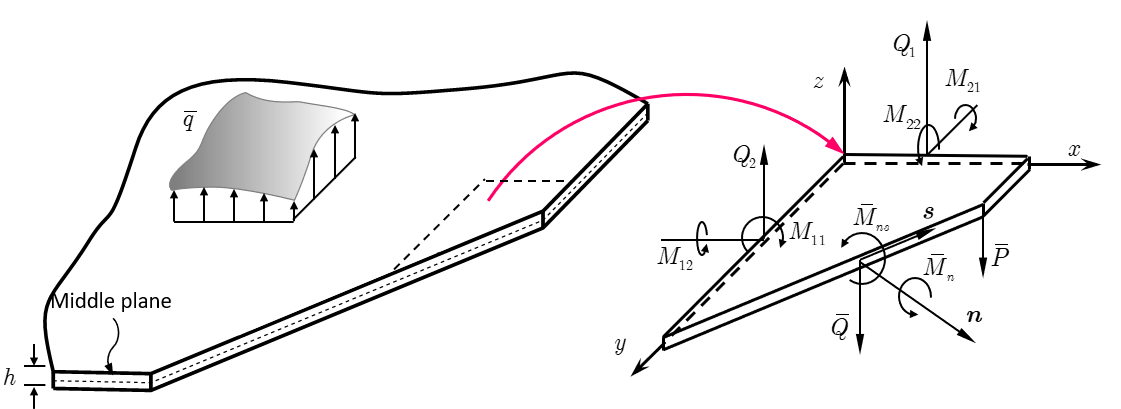
\includegraphics[scale=0.7]{figure/boban.png}
    \caption{薄板的相关符号及边界条件}
\end{figure}\newpage
\section{挠度离散和再生核近似}
本文针对Hellinger-Reissner伽辽金弱形式中的薄板挠度和弯矩分别采用不同的近似方案进行离散,其中挠度采用基于再生核近似的无网格形函数进行离散。首先,在薄板中面$\Omega$上布置一系列无网格节点$\{\pmb{x}_I\}_{I=1}^{n_p}$,薄板挠度$w$的近似表达式$w^h$及其虚位移$\delta w^h$可表示为:
\begin{equation}
    w^h(\pmb{x})=\sum_{I=1}^{n_p}\Psi_I(\pmb{x})d_I,\quad \delta w^h(\pmb{x})=\sum_{I=1}^{n_p}\Psi_I(\pmb{x})\delta d_I
\end{equation}
式中$d_{I}$、$\Psi_I(\pmb{x})$为无网格节点$\pmb{x}_I$上的节点系数和无网格形函数。根据再生核近似理论,无网格形函数可假设为如下表达式:
\begin{equation}\label{shapefunction}
    \Psi_I(\pmb{x})=\pmb{p}^T(\pmb{x}_I-\pmb{x})\pmb{c}(\pmb{x})\phi(\pmb{x}_I-\pmb{x})
\end{equation}
其中$\pmb{p}(\pmb{x})$为$p$阶单项式基函数向量:
\begin{equation}
    \pmb{p}(\pmb{x})=\{1,\;x,\;y,\;\dots,\;x^iy^j,\;\dotsb,y^p\}^T,\quad 0\le i+j\le p
\end{equation}
$\phi(\pmb{x}_I-\pmb{x})$为核函数,核函数决定了无网格形函数的光滑性和影响域。本文采用基于五次样条函数的矩形影响域核函数,其表达式为:
\begin{equation}
    \phi(\pmb{x}_I-\pmb{x})=\phi(r_x)\phi(r_y),\quad r_{\alpha}=\frac{x_{\alpha I}-x_{\alpha}}{s_{\alpha I}}
\end{equation}
\begin{equation}
    \phi(r_{\alpha})=\frac{1}{5!}\begin{cases}
        (3-3r)^5-6(2-3r)^5+15(1-3r)^5&r\le\frac{1}{3}\\
        (3-3r)^5-6(2-3r)^5&\frac{1}{3}<r\le\frac{2}{3}\\
        (3-3r)^5&\frac{2}{3}<r\le1\\
        0&r>1
    \end{cases}
\end{equation}
式中$s_{\alpha I}$为节点$\boldsymbol x_I$处坐标轴$x_\alpha$方向的影响域边长。 \par
另一方面,$\pmb{c}$为待定系数向量,其表达式可通过如下所示的一致性条件确定:
\begin{equation}\label{cc}
    \sum_{I=1}^{n_p}\Psi_I(\boldsymbol x)\boldsymbol{p}(\boldsymbol x_I-\boldsymbol x) = \boldsymbol{p}(\boldsymbol{0})
\end{equation}
将式(\ref{shapefunction})代入上式可得:
\begin{equation}
    \Psi_I(\pmb{x})=\pmb{p}^T(\pmb 0)\pmb{A}^{-1}(\pmb{x})\pmb{p}(\pmb{x}_I-\pmb{x})\phi(\pmb{x}_I-\pmb{x})
\end{equation}
其中$\pmb{A}(\pmb{x})$为矩量矩阵,其表达式为:
\begin{equation}
    \pmb{A}(\pmb{x})=\sum_{I=1}^{n_p}\pmb{p}(\pmb{x}_I-\pmb{x})\pmb{p}^T(\pmb{x}_I-\pmb{x})\phi(\pmb{x}_I-\pmb{x})
\end{equation}\par
图2为二维二次基函数无网格形函数,从图中可以看出,无网格形函数在全域上连续光滑,但在无网格节点处,无论节点在域内还是边界处,形函数都不具有插值性,因此无网格法中基本边界条件都需要特殊处理。
\begin{figure}[!h]
    \centering
    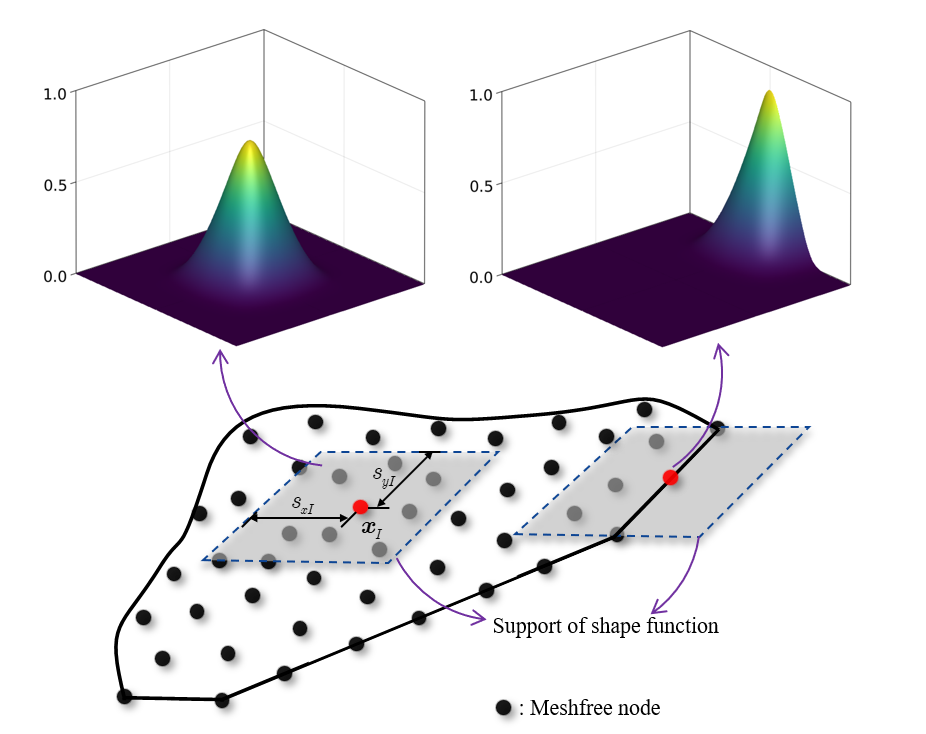
\includegraphics[scale=0.7]{figure/zaishenghe.png}
    \caption{无网格形函数}
\end{figure}\newpage
\section{弯矩离散和再生光滑梯度近似}
针对HR伽辽金弱形式中弯矩的近似,首先将薄板中面$\Omega$划分为一系列背景积分单元$\Omega_C$,$C=1,2,\dots,n_c$,并且有$\cup_{C=1}^{n_c}\Omega_C=\Omega$。在背景积分单元$\Omega_C$内,弯矩分量$M_{\alpha\beta}$的近似表达式$M^h_{\alpha\beta}$可表示为:
\begin{equation}\label{moment}
    M_{\alpha\beta}^h(\pmb{x})=\pmb{a}^T_{\alpha\beta}\pmb{q}(\pmb{x})
    % ,\delta \pmb M_{\alpha\beta}^h(\pmb{x})=\delta \pmb{a}^T_{\alpha\beta}\pmb{q}(\pmb{x}),\pmb{x}\in\Omega_C
\end{equation}
式中$\pmb{q}$为比$\pmb{p}$低两阶的单项式向量:
\begin{equation}
    \pmb{q}(\pmb{x})=\{1,\;x,\;y,\;\dots,\;x^iy^j,\;\dots,\;y^{p-2}\}^T,0 \le i+j \le p-2
\end{equation}
$\pmb a_{\alpha\beta}$是积分域$\Omega_C$的常系数向量,将近似的弯矩式(\ref{moment})代入式(\ref{weakform1})可以得到:
% \begin{equation}
%     \begin{split}
%         &\int_\Omega {\delta a_{\alpha\beta}^T{q}({x})D_{\alpha \beta \gamma \eta }^{ - 1}{a_{\gamma\eta}^Tq(x)}d\Omega }- \int_\Omega =\int_\Gamma  {\delta {V_{\bf{n}}}wd\Gamma }  - \int_\Gamma  {\delta a_{\bf{nn}}^Tq(x){w_{,{\bf{n}}}}d\Gamma }+{\left. {\delta Pw} \right|_{{\bf{x}} \in c}} \\
%         & -{\delta a_{\alpha\beta,\alpha\beta}^Tq(x)wd\Omega }-\int_{{\Gamma _w}} {\delta {V_{\bf{n}}}wd\Gamma }  + \int_{{\Gamma _\theta }} {\delta a_{\bf{nn}}^Tq(x){w_{,{\bf{n}}}}d\Gamma }  - {\left. {\delta Pw} \right|_{{\bf{x}} \in {c_w}}}\\
%         &+\int_{{\Gamma _w}} {\delta {V_{\bf{n}}}\bar wd\Gamma }  - \int_{{\Gamma _\theta }} {\delta a_{\bf{nn}}^Tq(x){{\bar \theta }_{\bf{n}}}d\Gamma }  + {\left. {\delta P\bar w} \right|_{{\bf{x}} \in {c_w}}}
%     \end{split}
% \end{equation}
\begin{equation}
    \begin{split}
        &\int_\Omega {\delta a_{\alpha\beta}^T{q}({x})D_{\alpha \beta \gamma \eta }^{ - 1}{a_{\gamma\eta}^Tq(x)}d\Omega }+\int_\Gamma  {\delta a_{\bf{nn}}^Tq(x){w_{,{\bf{n}}}}d\Gamma }+\int_\Omega  {\delta a_{\alpha\beta,\alpha\beta}^Tq(x)wd\Omega }\\
        &-\int_{{\Gamma _\theta }} {\delta a_{\bf{nn}}^Tq(x){w_{,{\bf{n}}}}d\Gamma }+\int_{{\Gamma _\theta }} {\delta a_{\bf{nn}}^Tq(x){{\bar \theta }_{\bf{n}}}d\Gamma }=\int_\Gamma  {\delta {V_{\bf{n}}}wd\Gamma }+{\left. {\delta Pw} \right|_{{\bf{x}} \in c}}\\
        &+\int_{{\Gamma _w}} {\delta {V_{\bf{n}}}wd\Gamma }-{\left. {\delta Pw} \right|_{{\bf{x}} \in {c_w}}}+\int_{{\Gamma _w}} {\delta {V_{\bf{n}}}\bar wd\Gamma } + {\left. {\delta P\bar w} \right|_{{\bf{x}} \in {c_w}}}
    \end{split}
\end{equation}
进一步得出常系数向量$\pmb{a}$的表达式:
\begin{equation}\label{ca}
    a_{\gamma\eta}=-D_{\alpha\beta\gamma\eta}G^{-1}(\sum_{I=1}^{n_p}(\tilde{g}_{\alpha\beta I}-\bar{g}_{\alpha\beta I})d_I+\hat{g}_{\alpha\beta})
\end{equation}
式中:
\begin{equation}
    G=\int_{\Omega_C}\pmb{q}\pmb{q}^Td\Omega
\end{equation}
\begin{equation}
\begin{split}
% \begin{cases}
    &{\tilde g}_{\alpha\beta I} = \int_{{\Gamma _C}}^{}{{\Psi _{I,{\bf{n}}}}{\pmb{q}}{n_\alpha }{n_\beta }d\Gamma }-\int_{{\Gamma _C}}^{}{{\Psi _I}({n_\alpha }{{\pmb{q}}_{,\beta }} + {{\pmb{q}}_{,\gamma }}{s_\alpha}{n_\beta }{s_\gamma})d\Gamma }  + {\left[\kern-0.15em\left[ {{\Psi _I}{\pmb{q}}{n_\alpha }{s_\beta }} 
     \right]\kern-0.15em\right]_{{{x}} \in {c_C}}} + \int_{{\Omega _C}}^{} {{\Psi _I}{{\pmb{q}}_{,\alpha \beta }}d\Omega } \\
    &{\bar g}_{\alpha \beta I} = \int_{{\Gamma _\theta } \cap {\Gamma _C}}^{} {{\Psi _{I,{\bf{n}}}}{\pmb{q}}{n_\alpha }{n_\beta }d\Gamma }  - \int_{{\Gamma _w} \cap {\Gamma _C}}^{} {{\Psi _I}({n_\alpha }{{\pmb{q}}_{,\beta }} + {{\pmb{q}}_{,\gamma }}{s_\alpha }{n_\beta }{s_\gamma })d\Gamma }  + {\left[\kern-0.15em\left[ {{\Psi _I}{\pmb{q}}{n_\alpha }{s_\beta }} 
     \right]\kern-0.15em\right]_{{{x}} \in {c_w} \cap {c_C}}}\\
    &\hat{g}_{\alpha \beta }= \int_{{\Gamma _\theta } \cap {\Gamma _C}}^{} {{\pmb{q}}{n_\alpha }{n_\beta }{{\bar \theta }_{\bf{n}}}d\Gamma }  - \int_{{\Gamma _w} \cap {\Gamma _C}}^{} {({n_\alpha }{{\pmb{q}}_{,\beta }} + {{\pmb{q}}_{,\gamma }}{s_\alpha }{n_\beta }{s_\gamma })\bar wd\Gamma }  + {\left[\kern-0.15em\left[ {\bar w{\pmb{q}}{n_\alpha }{s_\beta }} 
     \right]\kern-0.15em\right]_{{{x}} \in {c_w} \cap {c_C}}}
% \end{cases}
\end{split}
\end{equation}
其中,$\Gamma_C$是$\Omega_C$的边界。将式(\ref{ca})代入到式子(\ref{moment})中可以得到${M}^h_{\alpha\beta}$的表达式:
\begin{equation}
\begin{split}
M_{\alpha\beta}^h(x)&=q^T(x)a_{\alpha\beta}\\
&=-D_{\alpha\beta\gamma\eta}(\sum_{I=1}^{n_p}(q^T(x)G^{-1}\tilde{g}g_{\gamma\eta I}-q^T(x)G^{-1}\bar{g}_{\gamma\eta I})d_I+q^T(x)G^{-1}\hat{g}_{\gamma\eta})\\
&=-D_{\alpha\beta\gamma\eta}(\sum_{I=1}^{n_p}\tilde{\Psi}_{I,\gamma\eta}(x)d_I-\sum_{I=1}^{n_p}\bar{\Psi}_{I,\gamma\eta}(x)d_I+q^T(X)G^{-1}\hat{g}_{\gamma\eta})
\end{split}
\end{equation}
式中:
\begin{equation}
\begin{split}
\begin{cases}
    \tilde{\Psi}_{I,\alpha\beta}=q^T(x)G^{-1}\tilde{g}_{\alpha\beta I}\\
    \bar{\Psi}_{I,\alpha\beta}=q^T(x)G^{-1}\bar{g}_{\alpha\beta I}
\end{cases}
\end{split}
\end{equation}\par
通过对挠度和弯矩进行混合离散,可以得到离散控制方程:
\begin{equation}
\begin{split}
    \pmb{M}\ddot{\pmb d}+(\pmb{K}+\pmb{\tilde{K}}+\pmb{\bar{K}})\pmb{d}=\pmb{f}+\pmb{\tilde{f}}+\pmb{\bar f}
\end{split}
\end{equation}
其中:
\begin{equation}
\begin{split}
    &\pmb{K}_{I\!J}=\int_{\Omega}\tilde{\Psi}_{I,\alpha\beta}D_{\alpha\beta\gamma\eta}\tilde{\Psi}_{J,\gamma\eta}d\Omega\\
    &\pmb{M}_{I\!J}=\int_{\Omega}\Psi_I\rho h\Psi_Jd\Omega\\
    &\pmb{f}_I=\int_{\Gamma_V}\Psi_I\bar{V}_n\Gamma-\int_{\Gamma_M}\Psi_{I,n}\bar{M}_{nn}d\Gamma+\int_{\Omega}\Psi_I\bar{q}d\Omega+\Psi_I\bar{P}\vert_{x\in c_P}
\end{split}
\end{equation}
\begin{equation}
\begin{split}
   \pmb{\tilde{K}}_{I\!J}=\\
   \pmb{\tilde{f}}_I= 
\end{split}
\end{equation}
\begin{equation}
\begin{split}
     \pmb{\bar{K}}_{I\!J}=\\
     \pmb{\bar{f}}_I=
\end{split}
\end{equation}
\section{时间域离散}
本研究采用Newmark法对薄板控制方离散方程进行时间离散:\\
预测阶段:
\begin{equation}
\begin{split}
    \begin{cases}
        \tilde{\pmb{d}}_{n+1}=\pmb{d}_n+(\triangle t_n)v_n+\frac{\triangle (t_n)^2}{2}(1-2\beta)\pmb a_n\\
        \tilde{\pmb v_{n+1}}=\pmb{v}_n+(\triangle t_n)(1-\gamma)\pmb{a}_n
    \end{cases}
\end{split}
\end{equation}
矫正阶段:
\begin{equation}
\begin{split}
    \begin{cases}
    \pmb{d}_{n+1}=\tilde{d}_{n+1}+\beta(\triangle t_n)^2\pmb a_{n+1}\\
    \pmb v_{n+1}=\tilde{v}_{n+1}+\gamma(\triangle t_n)\pmb{a}_{n+1}
    \end{cases}
\end{split}
\end{equation}
其中,$\triangle t_n=t_{n+1}-t_n$,$\pmb{d}_n,\pmb{v}_n,\pmb a_n$表示为时刻为$t_n$的挠度,速度以及加速度。$\beta$和$\gamma$是Nemark参数。将矫正阶段的式子(29)带入到整体离散控制方程(23)可以通过满足一致性条件得到,进而可以得到无网格形函数表达式为:
\begin{equation}
\begin{split}
\pmb{M}+\beta(\triangle t_n)^2(\pmb{K}+\pmb{\tilde{K}}+\pmb{\bar{K}})\pmb{a}_{n+1}=\pmb{f}_{n+1}+\tilde{\pmb{f}}_{n+1}+\bar{\pmb{f}}_{n+1}-(\pmb{K}+\pmb{\tilde{K}}+\pmb{\bar{K}})\pmb{\tilde{d}}_{n+1}
\end{split}
\end{equation}
\section{数值算例}
\subsection{一维简支梁问题}
考虑如图1所示的一维简支梁问题,简支梁在跨中受到谐波点力$F(t)=F_0sin(wt)$,其中$\omega=\pi,F_0=10$。简支梁的几何和材料性质为:长度$L=10$,截面宽度$b=1$,厚度$t=1$,密度$\rho=2500$,一维简支梁的杨氏模量为$E=2\times10^6$。该问题的解析解为:
\begin{equation}
\begin{split}
    w(x,t) = \frac{{2{F_0}}}{{\rho AL}}\sum\limits_{i = 1,3,5...}^\infty  {(\sin (\frac{{i\pi }}{2})\frac{{\sin (i\pi x/L)}}{{{\omega ^2}_i - {\omega ^2}}} \times (\sin (\omega t) - \frac{\omega }{{{\omega _i}}}\sin ({\omega _i}t)))} \\ 
\end{split}
\end{equation}
其中
\begin{equation}
{\omega _i} = \frac{{{i^2}{\pi ^2}}}{{{L^2}}}\sqrt {\frac{{EI}}{{\rho A}}} 
\end{equation}
其中,$A=b\times h$表示为简支梁横截面的面积。\par
\begin{figure}[!h]
\centering
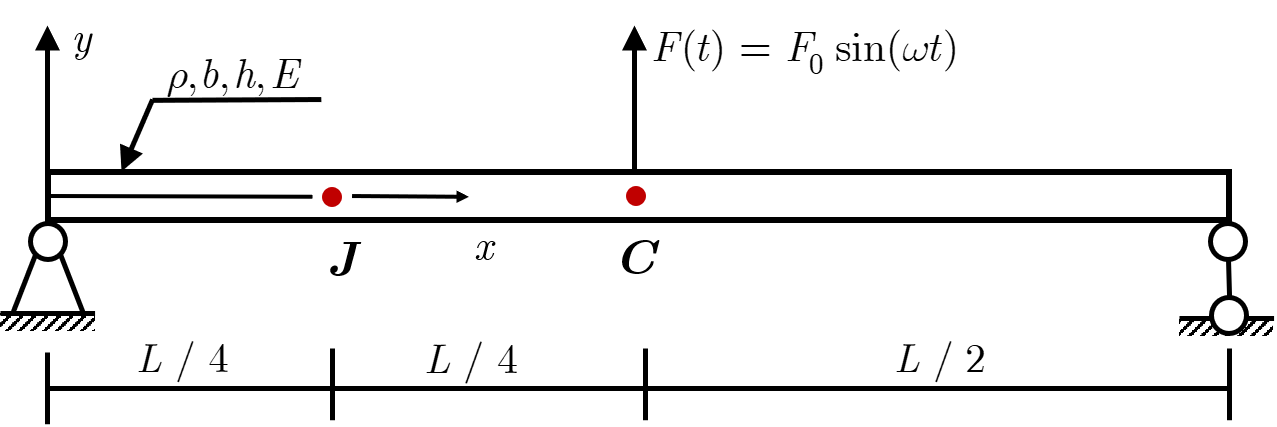
\includegraphics[scale=0.5]{figure/beam.png}
\caption{一维简支梁问题模型}
\end{figure}
\begin{figure}[!h]
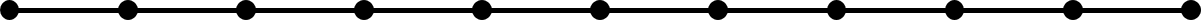
\includegraphics[scale=0.5]{figure/beam.mesh.png}
\caption{一维简支梁问题模型节点离散}
\end{figure}
一维简支梁的求解域以图2所示采用11个均匀间隔的节点进行离散分析,算例采用具有三次和四次基函数的无网格近似函数计算,核函数的相对影响域分别为3.5\\和4.5。时间设置步长为$\triangle t=0.01s$。
为了方便起见,定义挠度误差$error=\omega^h(x,t)-\omega^{\varepsilon}(x,t)$来定义各种方法的准确性,图和图分别表示的是一维简支梁模型采用三次和四次基函数中心点C的挠度时间历程和挠度误差,
从图3和图4可以清楚的看出采用RKGSI方法的解精度最好,挠度误差几乎为0,而采用GI-2和GI-5方法的误差几乎相同,相较于RKGSI-HR方法的误差较大,充分说明了RKGSI方法在频率计算方法的精确性。
\subsection{简支方板问题}
如图5所示,二维简支方板在板心$C$点处受到正弦集中力的作用,其中几何和材料参数为:长度为$a=10$,厚度$h=0.05$,密度$\rho=2\times 10^{11}$,泊松比$\nu=0.3$,集中力$F_0=1000$,频率$\theta=\pi$,
简支方板的精确解为:
\begin{equation}
\begin{split}
    w (x,y,t) = \mathop \sum \limits_{m = 1}^\infty  \mathop \sum \limits_{n = 1}^\infty  {W_m}_n(x,y){\eta _m}_n(t) 
\end{split}
\end{equation}
其中
\begin{equation}
\begin{split}
&{W_m}_n(x,y) = \frac{2}{{a\sqrt {\rho t} }}\sin (\frac{{m\pi x}}{a})\sin (\frac{{n\pi y}}{a})\\
&{\eta _m}_n(t) = \frac{{2{F_0}}}{{({\omega ^2}{{_m}_n} - {\theta ^2})a\sqrt {\rho t} }}\sin (\frac{{m\pi }}{2})\sin (\frac{{n\pi }}{2}) \times (\sin \theta t - \frac{\theta }{{{\omega _m}_n}}\sin {\omega _m}_nt)
\end{split}
\end{equation}
\begin{figure}[!h]
\begin{floatrow}
\ffigbox{\caption{简支方板问题模型}}{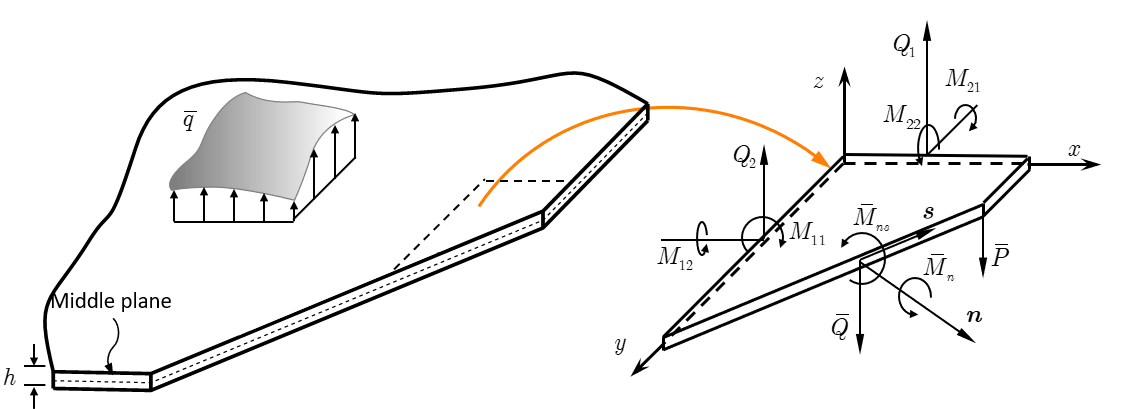
\includegraphics[scale=0.65]{figure/plate.png}}
\ffigbox{\caption{简支方板问题离散}}{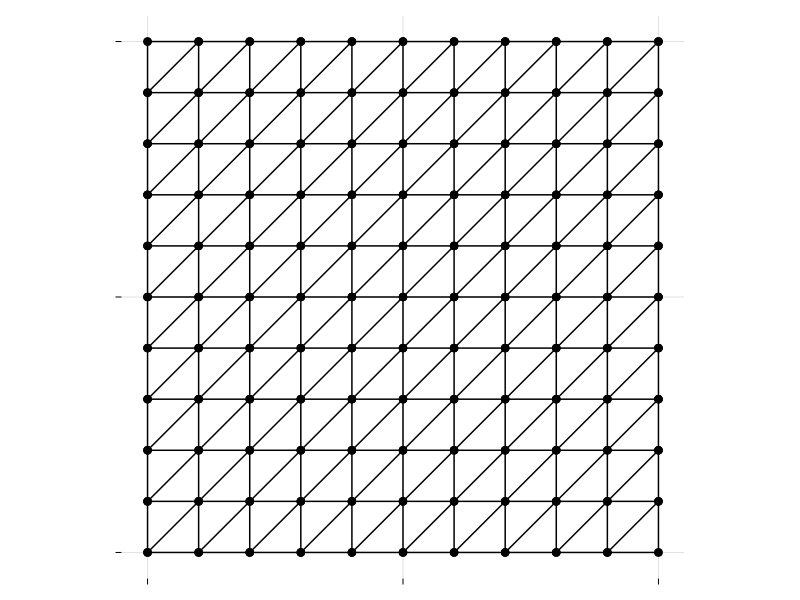
\includegraphics[scale=0.3]{figure/plate.mesh.png}}
\end{floatrow}
\end{figure}
简支方板的求解域根据图4所示的采用$11\times 11$的均匀间隔点进行离散分析,算例采用具有三次和四次基函数的无网格近似计算,核函数相对应的影响域分别为3.5和4.5。时间设置步长为$\triangle t=0.01s$。
图和图分别表示的是简支方板用三次和四次基函数时的中心点挠度的时间历程和挠度误差,结果表明在二维情况下采用RKGSI的方法中心挠度误差几乎为0,同时也小于采用高斯积分GI-2和GI-5所得出的挠度误差,
进一步说明了RKGSI-HR方法在计算高阶薄板问题频率计算方面的准确性。

\bibliography{reference}
\end{document}